\documentclass[conference]{IEEEtran}
\usepackage{amsmath,amsfonts}
\usepackage{algorithm, algpseudocode}
\usepackage{array}
\usepackage[caption=false,font=normalsize,labelfont=sf,textfont=sf]{subfig}
\usepackage{textcomp}
\usepackage{stfloats}
\usepackage{url}
\usepackage{verbatim}
\usepackage{graphicx}
\usepackage{cite}

\hyphenation{op-tical net-works semi-conduc-tor IEEE-Xplore}
% updated with editorial comments 8/9/2021

% \usepackage[style = numeric]{biblatex}
% \addbibresource{references.bib}

\bibliographystyle{unsrt}

\begin{document}


\title{Reinforcement Learning Project 2 Report\\ Lunar Lander}

\author{Xingyan Liu (202264690069@mail.scut.edu.cn), Shiyi Wang (202230055267@mail.scut.edu.cn) \\Wolin Liang (202264690304@mail.scut.edu.cn), Haoming Jia (202264690267@mail.scut.edu.cn) 
\\Instructor: Ou Shiqi
\thanks{Liu Xingyan: Responsible for code programming, results collation and analysis.Wang Shiyi: Focuses on literature research and problem modeling, specifically defining the problem environment.Liang Wolin: Handles the introduction of related work and paper analysis.Jia Haoming: Analyzes the experimental results and their significance.}% <-this % stops a space
\thanks{Manuscript revised November 10, 2024.}}

% The paper headers
\markboth{Group 1 for Reinforcement Learning, Fall~2024}%
{Shell \MakeLowercase{\textit{et al.}}: A Sample Article Using IEEEtran.cls for IEEE Journals}

\maketitle
\section*{Abstract}
\textbf{DQN, a model-free reinforcement learning approach, enables high-dimensional control by approximating the action-value function \( Q(s, a) \) and was implemented in the Lunar Lander environment with systematic hyperparameter tuning. We found that an epsilon decay of \( 0.995 \), a discount factor of \( \gamma = 0.99 \), and a learning rate of \( \alpha = 0.0005 \) yielded optimal results, enabling the agent to achieve a stable landing policy.}


\section{Introduction and related work}

During the Apollo lunar landings, the lunar module went through several key phases. First, the descent engines slowed down, allowing the module to hover above the lunar surface so that the astronauts could choose a suitable landing site. During this time, the attitude control system made fine adjustments through small nozzles to keep it level and aligned with the landing area. Once the landing site was selected, the lunar module slowly descended, and the thrust was gradually reduced to ensure a smooth contact. When it contacted the lunar surface, the shock absorbers on the landing legs absorbed the impact and ensured that the module was stable. These steps ensured that the lunar module landed safely and protected the astronauts and equipment.

In the Apollo program, engineers used a variety of classical control theories and algorithms to adjust the lunar module to achieve a safe landing. These methods include linear control systems\cite{ogata2010modern}, feedback control\cite{franklin2015feedback}, proportional-integral-derivative (PID) control\cite{astrom2010feedback}, state-space methods\cite{kailath1980linear}, Kalman filtering\cite{kalman1960new}, and optimal control theory\cite{kirk2004optimal}.However, these methods are still insufficient in adaptability and still rely heavily on manual operations in actual operations. Therefore, the problem of using reinforcement learning methods to control the landing capsule for soft landing is proposed\cite{brockman2016openai}.

The LunarLander environment in OpenAI Gym serves as a benchmark for evaluating the performance of various reinforcement learning algorithms. This environment presents a complex control problem involving high-dimensional state spaces and requires sophisticated strategies for successful landings. Several algorithms have emerged as particularly effective in tackling this challenge. 

One of the pioneering approaches is the Deep Q-Network (DQN) \cite{mnih2015human}, which combines deep learning with Q-learning to approximate the Q-function using neural networks. DQN has demonstrated success in handling high-dimensional state spaces and complex decision-making tasks, including those presented by the LunarLander environment. 

Variants of DQN, such as Double DQN \cite{van2016deep} and Dueling DQN \cite{wang2016dueling}, have further enhanced performance by addressing overestimation biases and improving learning efficiency. Proximal Policy Optimization (PPO) is another prominent algorithm, favored for its simplicity and robustness \cite{schulman2017proximal}. PPO utilizes a novel approach to policy gradient methods by constraining the policy updates, which results in more stable training processes. This stability has led to PPO achieving superior performance in environments like LunarLander. 

Furthermore, Deep Deterministic Policy Gradient (DDPG), typically applied to continuous action spaces, has been successfully adapted to the continuous version of LunarLander (LunarLanderContinuous-v2) \cite{lillicrap2015continuous}. DDPG's ability to handle continuous control problems makes it particularly suitable for fine-tuning the lander's control mechanisms. The success of these algorithms is largely attributed to their capability to manage high-dimensional state spaces and optimize complex strategies. Numerous open-source projects and tutorials have demonstrated the implementation and tuning of these algorithms within the LunarLander environment, providing valuable resources for further research and development. These contributions highlight the potential of reinforcement learning in solving intricate control problems and pave the way for future advancements in the field.

\section{Problem Modeling}

\subsection{Lunar Lander Environment}

The Lunar Lander environment features an 8-dimensional state vector \([x, y, v_x, v_y, \theta, v_\theta, \textit{left\_leg}, \textit{right\_leg}]\), where \( x \) and \( y \) denote the horizontal and vertical positions, \( v_x \) and \( v_y \) are the respective velocities, \( \theta \) represents the orientation angle, and \( v_\theta \) is the angular velocity of the lander. The binary variables \textit{left\_leg} and \textit{right\_leg} indicate whether each leg has made contact with the ground. The agent has four discrete actions: \textit{no\_action}, \textit{fire\_left}, \textit{fire\_right}, and \textit{fire\_main}. Firing the main engine incurs a penalty of -0.3 points, while using an orientation engine incurs -0.03 points per use. The task is considered solved when the agent achieves an average score of 200 points or higher over 100 consecutive episodes.



\subsection{Q-Learning Overview}

Q-learning is a model-free, off-policy RL algorithm that learns an action-value function \( Q(s, a) \), which represents the expected cumulative reward for taking action \( a \) in state \( s \). The Q-values are updated according to the Bellman equation:

\begin{equation}
Q(s, a) \leftarrow Q(s, a) + \alpha \left( r + \gamma \max_{a'} Q(s', a') - Q(s, a) \right)
\end{equation}
The parameters include the learning rate \( \alpha \in (0, 1] \), discount factor \( \gamma \in [0, 1] \), the immediate reward \( r \), and the maximum Q-value of the next state \( \max_{a'} Q(s', a') \).


The off-policy approach of Q-learning enables the agent to explore with an exploration policy while learning an optimal target policy, optimizing cumulative long-term rewards.
 

\subsection{Deep Q-Network (DQN) for Continuous State Spaces}

Given the continuous state space in Lunar Lander, maintaining a discrete Q-table is infeasible. Instead, a Deep Q-Network (DQN) is used, where a neural network approximates \( Q(s, a) \), enabling generalization across the high-dimensional state space. Key techniques for DQN stability include:

\begin{enumerate}
    \item \textit{Experience Replay}: Storing and randomly sampling from past experiences \((s, a, r, s')\) minimizes correlation between samples, promoting convergence.
    \item \textit{Target Networks}: A separate target network, updated periodically, helps mitigate feedback loops and stabilizes Q-value updates.
\end{enumerate}

\subsection{Hyperparameter Tuning}

\subsubsection{Epsilon Decay Rate}

The epsilon decay rate controls the trade-off between exploration and exploitation. Starting with a high \( \epsilon \) (e.g., 1.0), it decays over time to increase exploitation of learned knowledge:
\begin{equation}
\epsilon_t = \epsilon_0 \cdot \text{decay\_factor}^t,
\end{equation}
where \( \epsilon_0 \) is the initial exploration rate and \( \text{decay\_factor} \) (e.g., 0.995) adjusts \( \epsilon \) at each episode.

\subsubsection{Discount Factor \( \gamma \)}

The discount factor \( \gamma \in [0, 1] \) controls the weight of future rewards. Higher values (e.g., \( \gamma = 0.99 \)) prioritize long-term rewards, making it suitable for tasks with delayed objectives. The cumulative reward \( G_t \) at time \( t \) is defined as:
\begin{equation}
G_t = \sum_{k=0}^{\infty} \gamma^k r_{t+k+1}.
\end{equation}

\subsubsection{Learning Rate \( \alpha \)}

The learning rate \( \alpha \) dictates the extent of Q-value updates, balancing convergence speed and stability. The Q-value update is defined by:
\begin{equation}
Q(s, a) \leftarrow Q(s, a) + \alpha \cdot \delta,
\end{equation}
where \( \delta = \left( r + \gamma \max_{a'} Q(s', a') - Q(s, a) \right) \) is the temporal difference (TD) error. Proper tuning of \( \alpha \) is crucial for stable learning.





\section{Experiment and Results}
The DQN algorithm is based on off-policy Q-learning and combines function approximation with experience replay and target network stabilization techniques. Specifically, experience replay helps to decorrelate observations, while the use of a target network mitigates the risk of feedback loops during training, thus improving stability.

\subsection{Algorithm Overview}

	\begin{algorithm}[H]
		\caption{DQN Algorithm for Lunar Lander}
		\begin{algorithmic}
			\Require Environment $\mathcal{E}$, learning rate $\alpha$, discount factor $\gamma$, exploration rate $\epsilon$, decay rate, target update frequency $C$
			\Ensure Trained Q-network with optimal action-value function
			
			\State \textbf{Initialize:}
			\State Replay memory $D$ with capacity $N$
			\State Primary Q-network $Q$ with weights $\theta$
			\State Target Q-network $\hat{Q}$ with weights $\theta^{-} \leftarrow \theta$
			
			\For{each episode}
			\State Reset environment to get initial state $s_0$
			\For{each step in the episode}
			\State Select action $a_t$ as:
			\[ 
			a_t = 
			\begin{cases} 
				\text{random action,} & \text{with probability } \epsilon \\ 
				\arg\max_a Q(s_t, a; \theta), & \text{with probability } 1 - \epsilon 
			\end{cases}
			\]
			\State Execute $a_t$, observe reward $r_t$ and next state $s_{t+1}$
			\State Store transition $(s_t, a_t, r_t, s_{t+1})$ in $D$
			\If{$D$ has enough samples}
			\State Sample mini-batch $(s_j, a_j, r_j, s_{j+1})$ from $D$
			\State Compute target $y_j$ as:
			\[
			y_j = 
			\begin{cases} 
				r_j, & \text{if } s_{j+1} \text{ is terminal} \\ 
				r_j + \gamma \max_{a'} \hat{Q}(s_{j+1}, a'; \theta^{-}), & \text{otherwise} 
			\end{cases}
			\]
			\State Update $\theta$ by minimizing loss: $\left( y_j - Q(s_j, a_j; \theta) \right)^2$
			\EndIf
			\If{\text{step mod } $C = 0$}
			\State Update target network: $\theta^{-} \leftarrow \theta$
			\EndIf
			\EndFor
			\State Decay $\epsilon$ according to decay rate
			\EndFor
		\end{algorithmic}
	\end{algorithm}






\subsection{Network Architecture and Hyperparameters}
The neural network used for Q-value approximation has two hidden layers, each with 64 units, and ReLU activation functions. The hyperparameters are selected based on empirical results and prior studies on DQN performance in similar environments. The chosen values are as follows:
	\begin{table}[h]
		\centering
		\caption{Hyperparameter Values for DQN Training}
		\begin{tabular}{|c|c|}
			\hline
			\textbf{Hyperparameter} & \textbf{Value} \\
			\hline
			Learning Rate ($\alpha$) & 0.001 \\
			\hline
			Discount Factor ($\gamma$) & 0.99 \\
			\hline
			Exploration Rate ($\epsilon$) & 1.0 (initial) \\
			\hline
			Decay Rate & 0.995 \\
			\hline
			Replay Memory Size ($N$) & 100000 \\
			\hline
			Target Update Frequency ($C$) & 1000 steps \\
			\hline
			Batch Size & 64 \\
			\hline
		\end{tabular}
		\label{tab:hyperparams}
	\end{table}

\subsection{Results}
The training results show clear progress in the agent’s performance. Figure \ref{fig:training_scores}, early scores are highly variable and often negative, reflecting the agent's initial struggles. Over time, scores trend upward, frequently exceeding 200, indicating improved skill. Figure \ref{fig:mean_scores} confirms this, showing a steady rise in average scores, reflecting the agent's growing consistency. By the end, the agent reaches near-target scores, proving that the DQN algorithm and fine-tuning enabled it to learn an effective landing strategy. 

\begin{figure}[h]
    \centering
    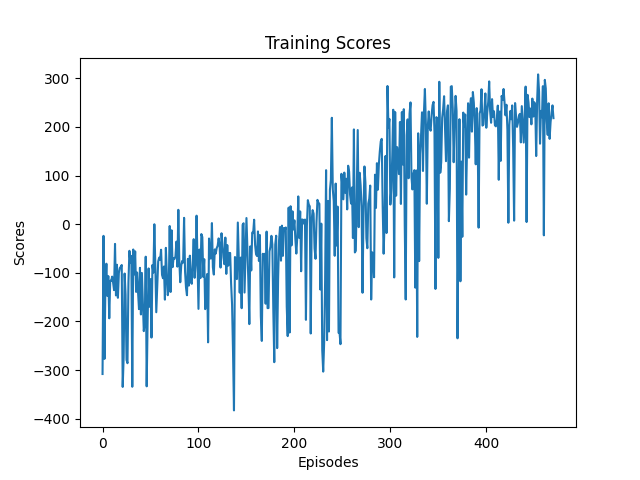
\includegraphics[width=0.5\textwidth]{Figure_1.png}
    \centering
    \caption{Training Scores over Episodes}
    \label{fig:training_scores}
\end{figure}

\begin{figure}[h]
    \centering
    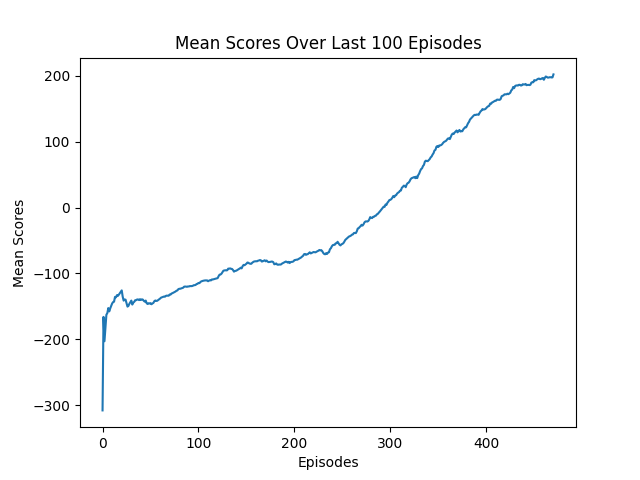
\includegraphics[width=0.5\textwidth]{Figure_2.png}
    \centering
    \caption{Mean Scores over the Last 100 Episodes}
    \label{fig:mean_scores}
\end{figure}


Additional experiments were performed to assess the impact of different hyperparameters, including epsilon decay, discount factors, and learning rates. The outcomes are presented in Figures \ref{fig:epsilon_decay_scores}, \ref{fig:gamma_scores}, and \ref{fig:learning_rate_scores}. 

\section{Result Analysis}

In this section, we analyze the experimental results in depth, with a focus on the effects of various hyperparameters such as epsilon decay, discount factor $\gamma$, and learning rate $\alpha$. 

\subsection{Impact of Epsilon Decay}

The epsilon decay rate controls the shift from exploration to exploitation by gradually reducing the likelihood of random actions as training progresses. As shown in Figure \ref{fig:epsilon_decay_scores}, a slower decay rate (e.g., 0.995) allowed the agent to explore thoroughly across various states before focusing on exploitation, leading to stable high performance in later episodes. In contrast, a faster decay rate (e.g., 0.8) led the agent to exploit prematurely, resulting in poorer performance due to insufficient exploration. These results suggest that a balanced epsilon decay rate, such as 0.995, optimally supports effective learning by enabling a gradual shift from exploration to exploitation.

\begin{figure}[h]
    \centering
    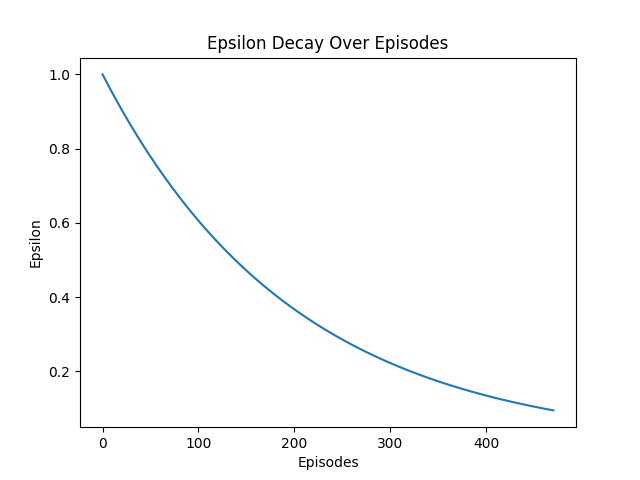
\includegraphics[width=0.5\textwidth]{Figure_3.png}
    \caption{Scores with Different Epsilon Decay Rates}
    \label{fig:epsilon_decay_scores}
\end{figure}

\subsection{Epsilon Decay Over Episodes}
The analysis in Figure \ref{fig:epsilon_decay_over_time} shows that the discount factor ($\gamma$) strongly affects the agent's stability and performance. Higher values, like $\gamma = 0.99$, lead to more consistent and higher scores, as they help the agent prioritize long-term rewards, which is crucial in complex tasks. Lower values, such as $\gamma = 0.5$, result in greater score variability and lower overall performance, reflecting a short-sighted strategy. Mid-range values show some improvement but lack the stability of the highest discount factor. Thus, a high discount factor proves effective for achieving a stable, high-performing policy.

\begin{figure}[h]
    \centering
    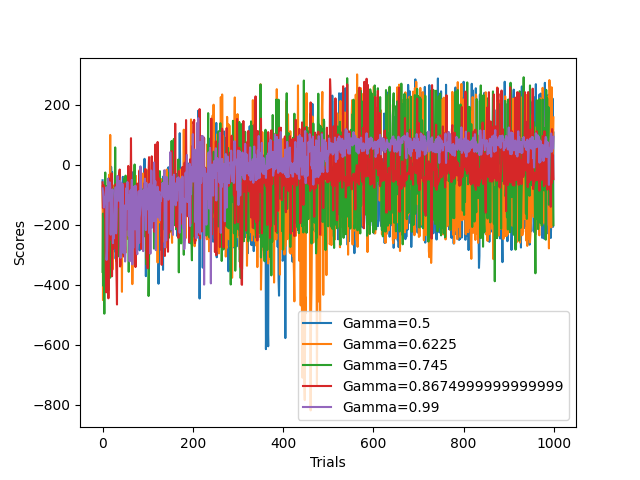
\includegraphics[width=0.5\textwidth]{Figure_6.png}
    \caption{Epsilon Decay Over Time for Different Decay Rates}
    \label{fig:epsilon_decay_over_time}
\end{figure}

\subsection{Impact of Discount Factor $\gamma$}
The discount factor $\gamma$ determines the extent to which future rewards are valued relative to immediate rewards. A high $\gamma$ value (e.g., 0.99) enables the agent to prioritize long-term rewards, which is essential in the Lunar Lander environment where optimal strategies often involve controlled, gradual maneuvers. Figure \ref{fig:gamma_scores} shows that epsilon decay rate strongly affects the agent’s performance. A slower decay rate (0.995) promotes balanced exploration, leading to higher and more stable scores as training progresses. This gradual shift from exploration to exploitation helps the agent develop a well-rounded policy. Faster decay rates (0.8 and 0.9), however, push the agent to exploit too soon, resulting in lower and more inconsistent scores. Thus, a decay rate of 0.995 appears optimal, providing enough exploration to support stable learning.

\begin{figure}[h]
    \centering
    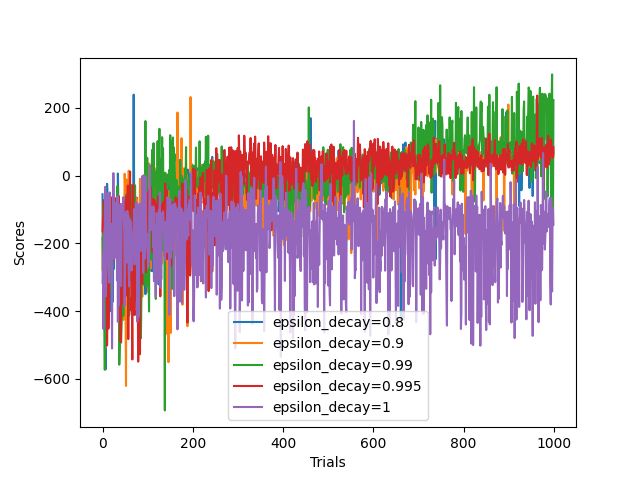
\includegraphics[width=0.5\textwidth]{Figure_4.png}
    \caption{Scores with Different Discount Factors}
    \label{fig:gamma_scores}
\end{figure}

\subsection{Impact of Learning Rate $\alpha$}
The learning rate $\alpha$ affects the speed and stability of the network's weight updates during training. As shown in Figure \ref{fig:learning_rate_scores}, an optimal learning rate of 0.0005 allowed the agent to converge efficiently while maintaining stability in the training process. Lower learning rates (e.g., $5 \times 10^{-5}$) led to slower convergence, as the updates to the Q-network were too small to capture the underlying dynamics of the environment effectively. On the other hand, excessively high learning rates (e.g., 0.05 or 0.5) introduced instability, with the agent frequently diverging from optimal policies and exhibiting large performance fluctuations. This observation aligns with standard DQN practices, suggesting that moderate learning rates are key to achieving a balanced convergence rate without sacrificing training stability.

\begin{figure}[h]
    \centering
    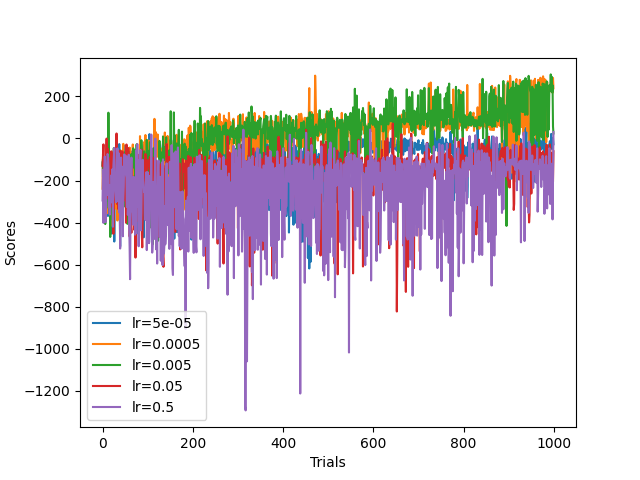
\includegraphics[width=0.5\textwidth]{Figure_7.png}
    \caption{Score Variability for Different Learning Rates}
    \label{fig:learning_rate_scores}
\end{figure}

Figure \ref{fig:epsilon_decay_rates} shows how different epsilon decay rates affect the transition from exploration to exploitation. Faster decay rates, like 0.8, reduce epsilon quickly, pushing the agent into exploitation early. Moderate rates (0.9 and 0.99) offer a more balanced shift. The slowest rate, 0.995, allows prolonged exploration, helping the agent learn a more stable policy. A rate of 1.0, with no decay, keeps the agent in constant exploration, hindering effective learning. Thus, a decay rate of 0.995 best supports a gradual and beneficial transition.

\begin{figure}[h]
    \centering
    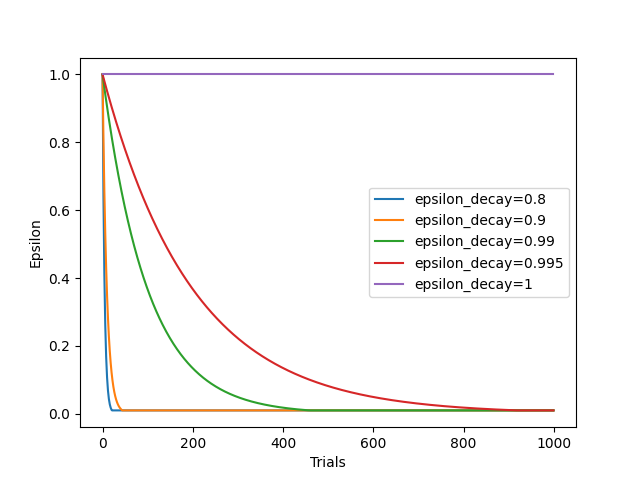
\includegraphics[width=0.5\textwidth]{Figure_5.png}
    \caption{Epsilon Per Training Trial Given Different Epsilon Decay Rates}
    \label{fig:epsilon_decay_rates}
\end{figure}


\subsection{Insights and Recommendations}
This analysis reveals key insights into how hyperparameter selection impacts DQN performance in continuous control tasks. A balanced epsilon decay rate, particularly around 0.995, is essential for thorough exploration in complex environments like Lunar Lander. This slower decay prevents premature convergence, allowing the agent to gather a richer set of experiences before prioritizing exploitation. A high discount factor ($\gamma = 0.99$) further supports stable, long-term policy optimization, which is advantageous in tasks requiring foresight. Together, these parameters promote the learning of robust, adaptable strategies.

Additionally, a moderate learning rate (0.0005) is crucial to achieving stable convergence. This rate effectively balances the speed of learning with stability, allowing the agent to capture environmental dynamics without risking divergence. Overall, the DQN agent effectively learns a policy for the Lunar Lander environment when hyperparameters are carefully tuned. Future work could enhance this approach by integrating advanced techniques, such as Dueling DQN and prioritized experience replay, to improve stability and accelerate learning. Testing the agent across varied scenarios could also provide insights into the generalizability and robustness of the learned policy.


% \vfill

\bibliographystyle{plain}
\bibliography{references}

\end{document}


